\documentclass{article}
\usepackage{amsmath} %This allows me to use the align functionality.
                     %If you find yourself trying to replicate
                     %something you found online, ensure you're
                     %loading the necessary packages!
\usepackage{amsfonts}%Math font
\usepackage{graphicx}%For including graphics
\usepackage{hyperref}%For Hyperlinks
\usepackage{listings}
\usepackage{graphicx}
\usepackage{natbib}        %For the bibliography
\bibliographystyle{apalike}%For the bibliography
\usepackage[margin=1.0in]{geometry}
\usepackage{float}
\begin{document}
%set the size of the graphs to fit nicely on a 8.5x11 sheet
\noindent \textbf{Caio Brighenti }\\
\noindent \textbf{COSC 302 - Analysis of Algorithms -- Spring 2019}\\%\\ gives you a new line
\noindent \textbf{Assignment 1}\vspace{1em}\\
\begin{enumerate}
	\item 
	Simply put, an algorithm is a way to solve a problem. In other words, it is a specific, well-defined step-by-step process to solve not just a single problem, but a category of similar problems. Algorithms must take some form of input, and must correctly use this input to solve its defined category of problems.
	\item 
	An example of a problem that cannot be solved is an algorithm that for any given input problem could output an efficient algorithmic solution to it. A similar scenario is NP-complete problems -- neither an algorithm nor a human has determined whether there are efficient solutions to this class of problems. There are plenty of problems for which we do not know efficient solutions, such as the Halting problem. An example of a non-algorithmic solution an algorithmically solvable problem would be the tallest student problem. We could simply look at the class and see quickly which student is the tallest, without systematically going one by one and comparing to the currently tallest -- we have an innate sense of things like this, and can process multiple pieces of information simultaneously, something a computer cannot do.
	\item The book defines analyzing an algorithm as predicting the resources that the algorithm requires, such as memory space, communication bandwith, or disk storage. Most commonly, it refers to analyzing the rate of growth of the algorithm's runtime, also known as time complexity.
	\item Each of the following are things that can be simplified when analyzing an algorithm \begin{itemize}
		\item 1 - Not specifying which case we are referring to and assuming worst
		\item 2 - Assuming each line is a single step
		\item 3 - Assuming the running time does not depend on the hardware
		\item 4 - Considering only the runtime with respect to the input and not other variables					
		\item 5 - Assuming that the biggest term in the running time dominates
		\item 6 - Assuming that each step takes the same amount of time
		\item 7 - Assuming that functions with the same dominating term are in the same category
		\item 8 - Ignoring the coefficients of the highest ordered term
		\item 9 - Not considering the actual runtime in a unit of time
		\item 10 - Assuming that the underlying hardware will execute a process step-by-step and not run in parallel
		\item 11 - Not clarifying if the complexity is different for the best case
		\item 12 - Not calculating the precise total of computer steps but just the order of growth
		\item 13 - Ignoring OS overhead like fetching things in memory or context swapping
		\item 14 - Considering only the time complexity and not the space complexity
	\end{itemize}
	\item The running time of an algorithm is a function that counts the number of steps the algorithm must execute as a function of the size of the input. If we re asked to calculate, we must ask whether we want the worst case, best case, or average case because there are different. If none of these are specified, then by convention we look at the worst case of the algorithm.
	\item The order of growth results from a simplification of the runtime. The order of growth relates to how the running time grows as a function of n, but we simplify and keep only the largest, dominating term, and we place all functions with the same simplified order of growth into a category. We can say that running time relates to an algorithm, while order of growth represents a category of algorithms.
	\item We typically use big-O more than other asymptotic notations for two reasons. Firstly, it provides us with information about the upper bound of the algorithm, meaning the maximum time it can take to run. This information is more important than the lower bound, as we would like to know what the slowest our algorithm can run is. Secondly, it is easier to determine big-O than Theta, as it provides information about only one bound, not both the upper and lower. Thus, big-O is used for its generality -- it is less specific than the other notations but provides us with the information we need to know.
	\item We say that an efficient algorithm is anything better than an exponential runtime, so typically polynomial or better. Of course, this measure is subjective, and it is possible that although we have an efficient solution for a problem, we might not have the most efficient solution.
	\item Not necessarily. If $f(n)$ is equal to $g(n)$, then the first part of the claim would be true, but $f(n)$ would not be asymptotically smaller than $g(n)$.
	\item Show by definition 
		\begin{enumerate}
			\item $f(n)\in \omega (g(n)) \implies f(n) \in \Omega (g(n))$
			\\ \\ By definition, if we have $f(n)\in \omega (g(n))$ then we have:
			\\ $g(n) \in o(f(n))$, and consequently:
			\\ $0\leq c_1g(n) < f(n)$
			\\ \\ The definition of $f(n) \in \Omega (g(n))$ is $0\leq c_1g(n) \leq f(n)$. Since for any $(x,y)$, $x<y \implies x\leq y$, then if we have:
			\\ $0\leq c_1g(n) < f(n)$
			\\ we must also have:
			\\ $0\leq c_1g(n) \leq f(n)$
			\\ Thus, the definition $f(n) \in \Omega (g(n))$ is met, and so the claim must be true.
			\item $f(n) \in \Theta (g(n)) \iff g(n)\in \Omega (f(n))$
			\\\\ If we have $f(n) \in \Theta (g(n))$, then by definition we have:
			\\ $0 \leq c_1g(n) \leq f(n) \leq c_2g(n)$
			\\ We then rearrange and combine each side of the inequality as follows. First, the left side:
			\begin{align}
				0 &\leq c_1g(n) \leq f(n) && \text{definition} \\
				0 &\leq g(n) \leq \frac{1}{c_1}f(n) && \text{divide by $c_1$}
			\end{align}
			\\ Then, the right side:
			\begin{align}
				f(n) \leq c_2g(n) && \text{definition} \\
				\frac{1}{c_2}f(n) \leq g(n) && \text{divide by $c_2$}
			\end{align}
			\\ Combining these two inequalities, we have:
			$$0 \leq \frac{1}{c_2}f(n) \leq g(n) \leq \frac{1}{c_1}f(n)$$
			\\ As $\frac{1}{c_1}$ and $\frac{1}{c_2}$ are both constants, then this meets the definition of $g(n) \in \Theta(f(n))$. Thus, $f(n) \in \Theta(g(n)) \implies g(n) \in \Theta(f(n))$ for all $n>n_0$.
			\\ Finally, we must show that this is two sided ($\iff$, not $\implies$). This is done simply by swapping $f(n)$ with $g(n)$ in the proof above. We arbitrarily selected $f(n)\in \Omega(g(n))$ as the starting point, and the math is identical if we do the opposite. Thus, the claim must be true.
		\end{enumerate}
	\item Using limit prove $2^n \in o(n!)$
	\\ We use Stirling's approximation to rewrite the second term such that:
	\begin{align}
		\lim_{n\to\infty}\frac{2^n}{n!} &= \lim_{n\to\infty} \frac{2^n}{\sqrt{2\pi n} (\frac{n}{e})^n}\\
		&=\lim_{n\to\infty} (\frac{2e}{n})^n \frac{1}{\sqrt{2\pi n}}
	\end{align}
	As the right term in the limit is a fraction with a constant numerator and a denominator that goes to $\infty$, then the term goes to 0 and can be eliminated. We then consider the left term. First, we let $y = (\frac{2e}{n})^n$. Then,
	\begin{align}
		\ln(y) &= n \ln(\frac{2e}{n}) \\
		\lim_{n\to\infty} \ln(y) &=\lim_{n\to\infty} n \ln(\frac{2e}{n}) \\
		&= \lim_{n\to\infty} \frac{\ln \frac{2e}{n}}{\frac{1}{n}} 
	\end{align}
	Now we consider a variable $x$ such that $x=\frac{1}{n}$. Since we are taking the limit of $n$ with respect to $\infty$, then $x$ will be going to 0. Thus, we now have a limit as $x$ goes to 0.
	\begin{align}
		\lim_{x\to 0} \frac{\ln 2ex}{x} &= \\
		&= \frac{-\infty}{0} \\
		&= -\infty
	\end{align}
	This is because $ln(x)$ approaches $-\infty$ as $x$ approaches 0. Thus, we have:
	\begin{align}
		\lim_{n\to\infty} \ln y &= \lim_{n\to\infty} \frac{ln \frac{2e}{n}}{\frac{1}{n}} = \lim_{x\to 0} \frac{\ln 2ex}{x} = -\infty\\
		\lim_{n\to\infty} \ln y &= -\infty
	\end{align}
	Finally, we use the property:
	$$\lim_{n\to\infty} \ln y = a \implies \lim_{n\to\infty} y = e^a$$
	\\ to determine $\lim_{n\to\infty} y$, where $y=(\frac{2e}{n})^n$ and $a=-\infty$.
	\begin{align}
		\lim_{n\to\infty} y &= e^a \\
		&= e^{-\infty} \\
		&= 0
	\end{align}
	Finally, let us rewrite the original full limit and plug in the separate limit terms calculated.
	\begin{align}
		\lim_{n\to\infty} \frac{2^n}{n!} &= \lim_{n\to\infty} (\frac{2e}{n})^n \frac{1}{\sqrt{2\pi n}} \\
		&= 0 \cdot 0 \\
		\lim_{n\to\infty}\frac{2^n}{n!} &= 0
	\end{align}
	Thus, we have that $2^n \in o(n!)$.
	\item Prove $f(n) \in o(g(n)) \implies f(n) + g(n) \in \Theta(g(n))$
	\\ Using the definitions of $o(n)$ and $\Theta(n)$ we can rewrite the claim as follows:
	\\	
	\\$0 \leq f(n) < c g(n) \implies 0 \leq c_1g(n) \leq f(n) + g(n) \leq c_2 g(n)$
	\\ For all $n>n_0$, and where $c$, $c_1$ and $c_2$ are positive constants. 
	\\ \\ We start by assuming the left side of the claim is true. Thus, since $f(n) < cg(n)$, then it must be that $cg(n)+f(n)\leq 2g(n)$, and that $g(n)\leq g(n)+f(n)$. Thus, we have:
	\begin{align}
	c(g(n)) + f(n) \leq 2g(n) &\leq 2(g(n) + f(n))\leq 4g(n) \\
	2g(n) &\leq 2(g(n) + f(n))\leq 4g(n)  && \text{eliminate left-most term}\\
	1g(n) &\leq g(n) + f(n)\leq 2g(n) && \text{divide by 2}
	\end{align}
	Thus, we have that $0 \leq c_1g(n) \leq f(n) + g(n) \leq c_2 g(n)$, where $c_1=1$ and $c_2=2$, for all $n>n_0$. Therefore, the claim must be true. 
	\\ \\ \textbf{Then, use this property find the asymptotic relation between:} 
	\\$f(n) = n+logn$ and $g(n) = 100n + log^2n$
	\\ First, we find the relationship between each of the terms in $f(n)$ and $g(n)$. We do this by first plotting $n$ vs $log(n)$, and then $100n$ versus $log^2n$. The plots are included below: \\
	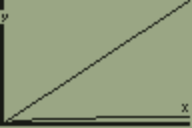
\includegraphics[scale=0.7]{12pt1.png}
	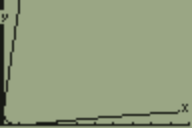
\includegraphics[scale=0.7]{12pt2.png}
	\\ On the left is the plot of $n$ versus $log(n)$, and $n$ clearly dominates asymptotically. Similarly, on the right $100n$ dominates $log^2(n)$. Thus, using the property we just proved, it must be that:
	\\ $f(n)\in \Theta (n)$
	\\ and 
	\\ $g(n)\in \Theta (100n) = \Theta(n)$
	\\ Thus, since both of the functions are linear, then it must be that $f(n) \in \Theta (g(n))$, or that $g(n) \in \Theta (f(n))$.
	\item Show order of growth between $n^3$ and $\log n^{\log n}$
	\\\\ We proceed by solving the limit $L = \lim_{n\to\infty} \frac{n^3}{(\log n)^{\log n}}$
	\\ First, we define a variable $y$ such that $y=\log n$. As $\log n$ will go to infinity as $n$ goes to infinity, we can instead the limit as $y$ approaches infinity. Additionally, if $y=\log n$, then we can rewrite $n^3$ as follows.
	\begin{align}
		\log n &= y \\
		n &= 2^y  \\
		n^3 &= (2^y)^ 3 = 2^{3y}
	\end{align}
	Thus, we rewrite and solve the limit as follows.
	\begin{align}
		L &= \lim_{y\to\infty} \frac{2^{3y}}{y^y} \\
		&= \lim_{y\to\infty} \frac{8^y}{y^y} \\
		&= \lim_{y\to\infty} (\frac{8}{y})^y
	\end{align}
	We now define a variable $Y$ such that $Y = (\frac{8}{y})^y$. Thus, we have that $\ln Y = y \ln \frac{8}{y}$. We then take the limit with respect to $\ln Y$ as $y$ approaches infinity.
	\begin{align}
		\lim_{y\to\infty} \ln Y &= \lim_{y\to\infty} y \ln \frac{8}{y} \\
		&= \lim_{y\to\infty} \frac{\ln \frac{8}{y}}{\frac{1}{2}} \\
		&= \frac{- \infty}{0} \\
		&= - \infty
	\end{align}
	This is because $\ln(x)$ goes to negative infinity as $x$ approaches 0, and both $\frac{8}{y}$ and $\frac{1}{y}$ will approach 0, as in both cases the numerator is a constant and the denominator goes to infinity.
	\\ Finally, we use the property:
	$$\lim_{n\to\infty} \ln y = a \implies \lim_{n\to\infty} y = e^a$$
	To determine the limit $\lim_{y\to\infty} Y$, where $a= - \infty$.
	\begin{align}
	\lim_{y\to\infty} Y &= e^a \\
	&= e^-\infty \\
	&= 0
	\end{align}
	Thus, rewriting the original limit and combining with this result, we have the following.
	\begin{align}
		\lim_{y\to\infty} \frac{n^3}{(\log n)^{\log n}} &= \lim_{n\to\infty} (\frac{8}{y})^y = 0 \\
		\lim_{y\to\infty} \frac{n^3}{(\log n)^{\log n}} &= 0
	\end{align}
	Thus, we have that $(\log n)^{\log n} \in \Theta (n^3)$.
	\item Rank the following functions by order of growth
	\\ I accomplished this problem by first guessing a potential order based on intuition (for instance, $n^2$ obviously grows slower than $2^n$). Then, I used a graphic calculator to plot each of the functions I thought to be close to each other, rearranging my initial based on the result. I plotted each function at least once, but I used the transitive property to assume that if $g_1=\Omega (g_2)$ and $g_2=\Omega (g_3)$ then $g_1=\Omega (g_3)$. For instances where the graphs were unclear, I calculated the limit between the two functions. Eventually, I obtained the following order, from largest to smallest.
	\begin{enumerate}
		\item $2^{2n+1}$
		\item $2^{2n}$
		\item $(n+1)!$
		\item $n!$
		\item $e^n$
		\item $n2^n$
		\item $2^n$
		\item $(\frac{3}{2})^n$
		\item $(\log n)^{\log n}$, $n^{\log \log n}$
		\item $n^3$
		\item $(\log n)!$
		\item $n^2$, $4^{\log n}$
		\item $n \log n$, $\log (n!)$
		\item $n$, $2^{\log}n$
		\item $\sqrt{2}^{\log n}$
		\item $(\log n)^2$
		\item $2^{\sqrt{2\log n}}$
		\item $\ln n$
		\item $\sqrt{\log n}$
		\item $\ln \ln n$
		\item $n^{\frac{1}{\log n}}$, $1$
	\end{enumerate}
\end{enumerate}
	

\end{document}
